\ylDisplay{Drooni vari} % Ülesande nimi
{Autor} % Autor
{lõppvoor} % Voor
{2017} % Aasta
{P 10} % Ülesande nr.
{3} % Raskustase
{
% Teema: Mehaanika

\ifStatement
Õhtusel ajal seisab Juku tenniseväljaku ääres, mille laius on $a $ning vaatleb, kuidas tema sõber lennutab drooni. On teada, et drooni kiiruse horisontaalkomponent on kogu lennu vältel $v$ ning horisontaalkomponendi suund ei muutu. Samuti on teada, et Päike asub otse drooni taga ja päikesekiired langevad maapinnale maapinna suhtes nurga $\alpha$ all. Algul lendab droon ühtlase kiirusega $v$ paralleelselt maapinnaga. Drooni vari ületab tenniseväljaku ajaga $t_1$. Droon jätkab lendamist sirgjoonelisel trajektooril, kuid mitte enam paralleelselt maapinnaga. Drooni vari liigub uuesti üle tenniseväljaku, nüüd eelnevaga vastassuunas. Teisel juhul ületab vari tenniseväljaku ajaga $t_2$. Kui palju muutus drooni lennukõrgus $h$ ajavahemiku $t_2$ jooksul?
\fi

\ifHint
Ülesande lahendamiseks tee abistav joonis, mis kuvab drooni liikumise trajektoori ning varju liikumist maapinnal. Ülesande lahendus peitub täisnurksete kolmnurkade lahendamises.
\fi

\ifSolution
\begin{center}
	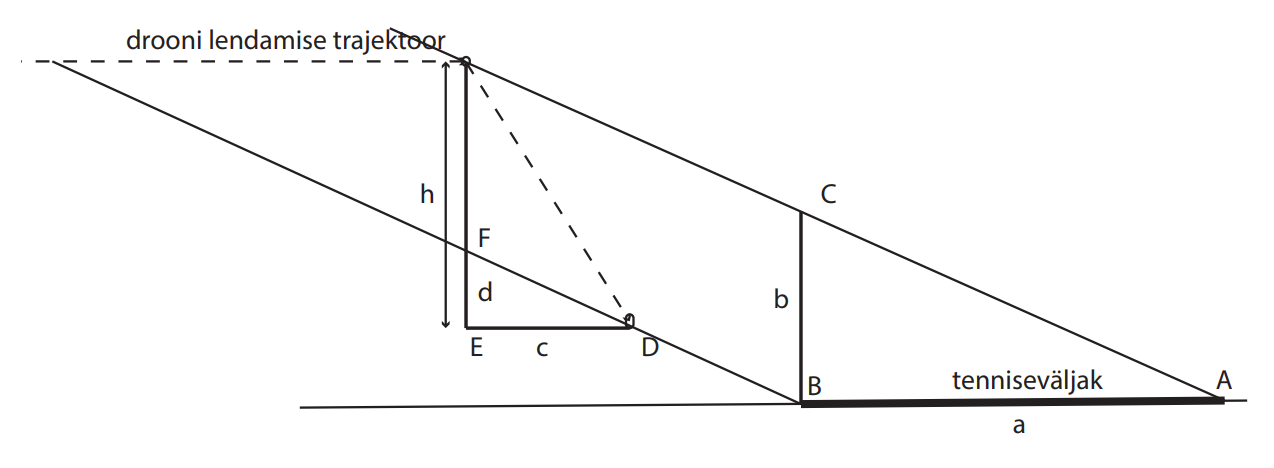
\includegraphics[width=0.5\linewidth]{2017-v3p-10-lah.PNG}
\end{center}
Paralleelselt maapinnaga lennates liigub drooni vari punktis $B$ punkti $A$. Kui droon laskub ja jõuab punkti $D$, siis drooni vari liigub laskumise ajal punktist $A$ punkti $B$.
Lennukõrguse muutus $h$ on lõikude $b$ ja $d$ summa. Kolmnurgast $\triangle ABC$  saame kätte kõrguse $b$.
\begin{center}
$tan\alpha = \frac{b}{d} \Rightarrow b = atan\alpha$
\end{center}
Kolmnurgast $\triangle DEF$ saame kätte kõrguse $d$
\begin{center}
$tan\alpha = \frac{d}{c} \Rightarrow d=ctan\alpha$
\end{center}
Drooni horisontaalne kiirus on kogu lennu ajal $v$. Algul ületas droon lennuväljaku ajaga $t_1$, seega 
\begin{center}
$b = vt_1 tan\alpha$. 
\end{center}
Tagasilenul oli drooni lennuaeg $t_2$, seega 
\begin{center}
$d = vt_2tan\alpha$
\end{center}
Droooni lennukõrguse muutus $h$ on seega 
\begin{center}
$h = b + d = vtan\alpha (t_1 + t_2) $
\end{center}
\fi
}